\documentclass[t,11pt]{beamer}
\usepackage{bjtu}
\usepackage{graphicx}
\graphicspath{ {./images/} {./logo/}}
\usepackage{caption}
\usepackage{booktabs}

%================在每个章节前显示目录==============
\AtBeginSection[]
{
  \begin{frame}
    \frametitle{Table of Contents}
    \setcounter{tocdepth}{1} % 显示一级标题
    \tableofcontents[currentsection]
  \end{frame}
}

%===================================================
%===============在这里修改标题和姓名================
%===================================================
\title{Title}
\author{Xuyang Cao}
\date{}

%====================文章主体=======================
\begin{document}

%========================标题页=====================
\frame{\titlepage}                  

%========================LOGO=======================
\logo{
\includegraphics[width=1cm,height=1cm]{logo_bjtu}\hspace{1.05\textwidth}\vspace{240pt}}

%========================目录页=====================
% 如果没有目录结构就注释掉
\begin{frame}{Table of Contents}           % table of contents frame 
    \setcounter{tocdepth}{1}               % 只显示一层目录结构
    \tableofcontents                       % table of contents
\end{frame}

%========================正 文======================
% 到对应的tex文件中编辑
\section{Section 1}
\begin{frame}[c]{Test Frame} % 参数c表示内容垂直居中,默认是顶部对齐[t]
    这是参考文献测试\cite{Cheplygina2018NotsosupervisedAS}
    
    这是一段中文测试
    
    公式:
    \[Dice = \frac{2 |A \cap B|}{|A| + |B|}\]
\end{frame}
 
\section{Section 2}
\begin{frame}[c]{Frame Title}
    \begin{columns}
    \column{0.5\textwidth}
    This is a text in first column.
    $$E=mc^2$$
    \begin{itemize}
    \item First item
    \item Second item
    \end{itemize}
     
    \column{0.5\textwidth}
    This text will be in the second column
    and on a second tought this is a nice looking
    layout in some cases.
    \end{columns}
\end{frame}


\begin{frame}{Frame Title}

\begin{columns}
\column{0.5\textwidth}
\begin{figure}
    \centering
    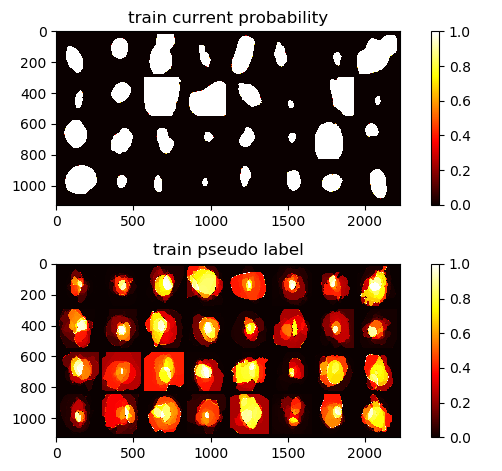
\includegraphics[width=1.\textwidth]{images/before.png}
    \caption*{Before}
\end{figure}

\column{0.5\textwidth}
\begin{figure}
    \centering
    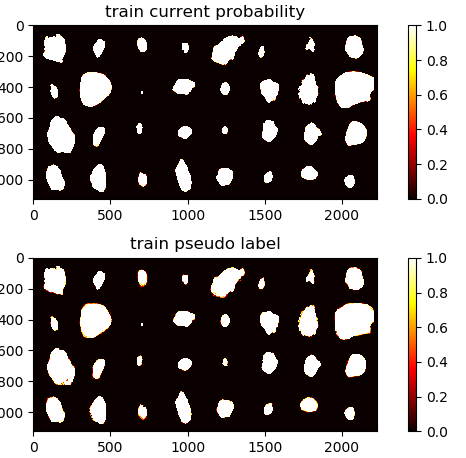
\includegraphics[width=1.\textwidth]{images/after.png}
    \caption*{After}
\end{figure}
\end{columns}
\end{frame}

\subsection{subsection 1} 

%=======================参考文献====================
% 如果不需要参考文献就注释掉
\begin{frame}{Reference}
    \bibliographystyle{ieeetr}
    \small\bibliography{references}
\end{frame}

\end{document}